\documentclass{article}

\usepackage{blindtext}
\usepackage{graphicx}
\usepackage{subcaption}
%\usepackage{subcaptions}

\pagenumbering{gobble}

\begin{document}

\title{carica e scarica di un condensatore}
\author{Ionut Cicio 3Binf.}
\date{02/02/2020}

\maketitle

\section*{Obiettivo}
\blindtext[1]

\section*{Strumenti}
\blindtext[1]

\newpage
\section*{Spiegazione teorica}
\subsubsection*{funzionamento}
\blindtext[1]
\subsubsection*{formule e grafici}
\blindtext[1]

%\caption{caption}
%\label{fig:label}

\newpage

\section*{circuito di carica}

\begin{figure}[h!]
  \centering
  \begin{subfigure}[b]{0.3\linewidth}
    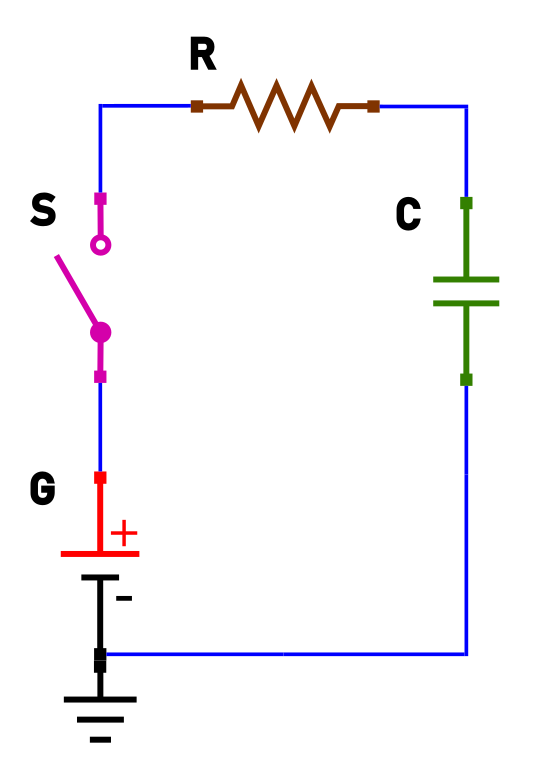
\includegraphics[width=\linewidth]{data/carica-open.png}
  \end{subfigure}
  \begin{subfigure}[b]{0.3\linewidth}
    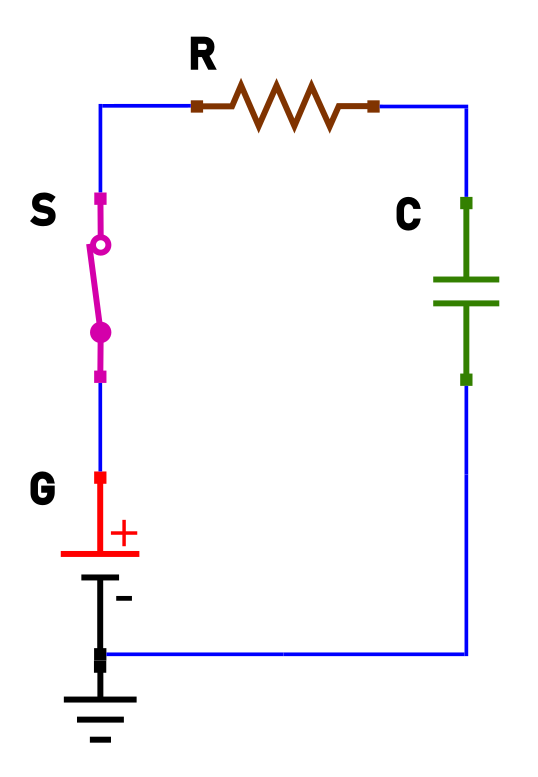
\includegraphics[width=\linewidth]{data/carica-closed.png}
  \end{subfigure}
  \begin{subfigure}[b]{0.347\linewidth}
    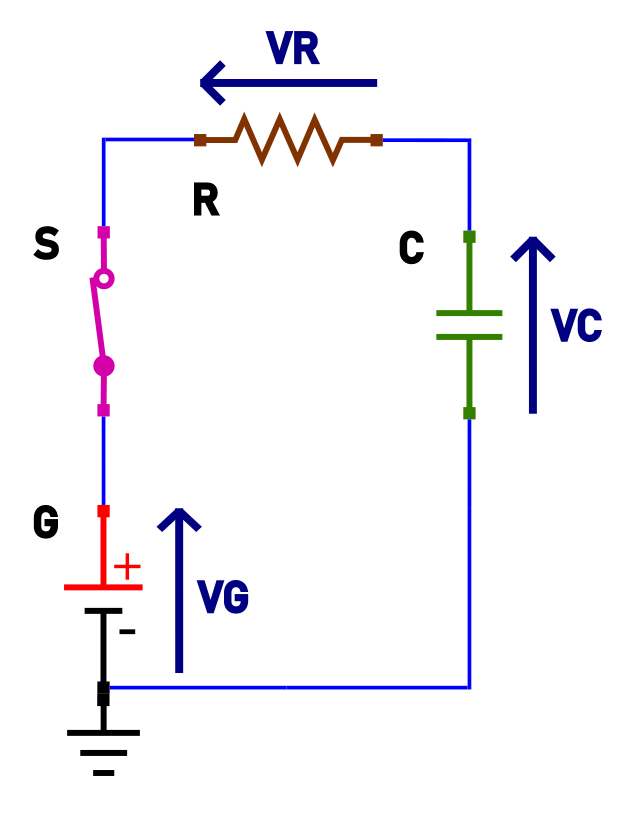
\includegraphics[width=\linewidth]{data/carica-tensioni.png}
  \end{subfigure}
\end{figure}

\subsubsection*{grafici carica}
\begin{figure}[h!]
  \centering
  \begin{subfigure}[b]{0.3\linewidth}
    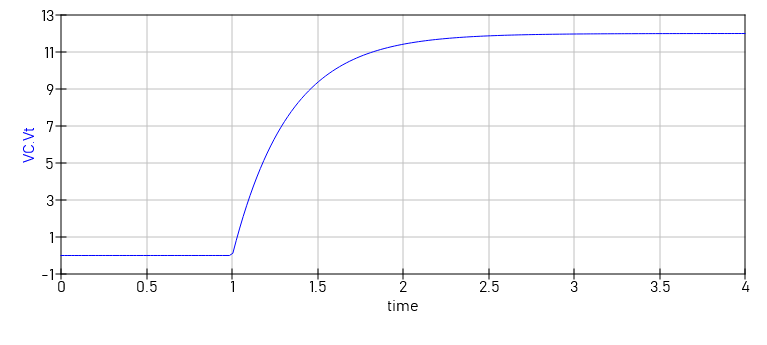
\includegraphics[width=\linewidth]{data/carica-VC.png}
  \end{subfigure}
  \begin{subfigure}[b]{0.3\linewidth}
    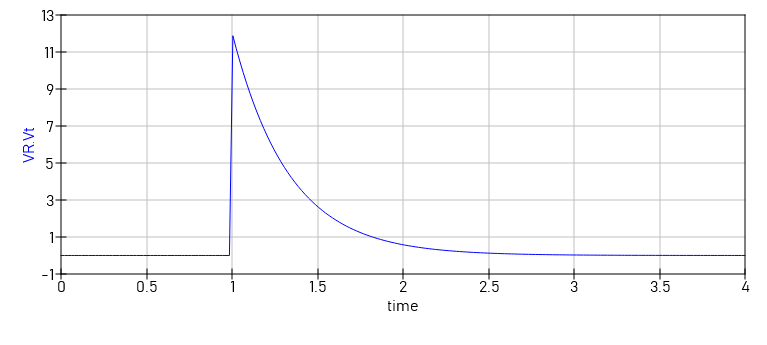
\includegraphics[width=\linewidth]{data/carica-VR.png}
  \end{subfigure}
  \begin{subfigure}[b]{0.3\linewidth}
    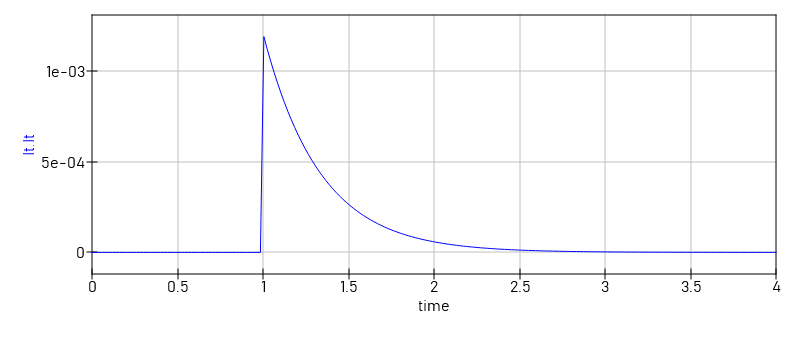
\includegraphics[width=\linewidth]{data/carica-IT.png}
  \end{subfigure}
\end{figure}


\newpage
\section*{circuito di sarica}

\begin{figure}[h!]
  \centering
  \begin{subfigure}[b]{0.3\linewidth}
    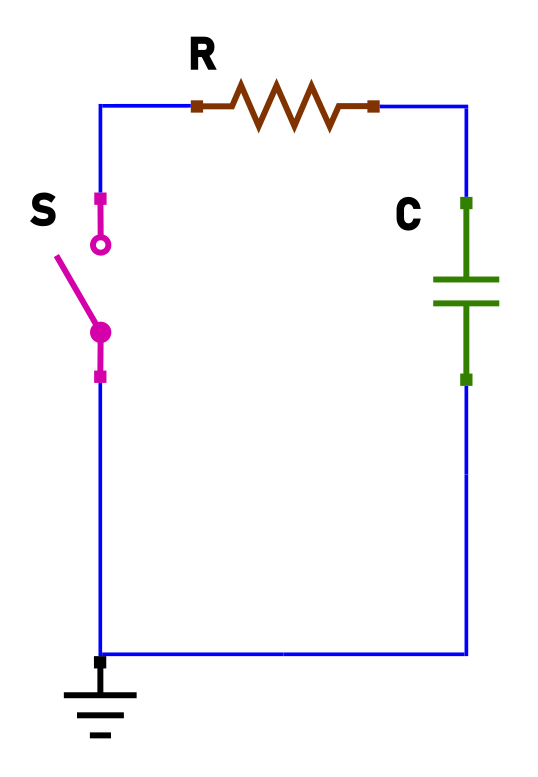
\includegraphics[width=\linewidth]{data/scarica-open.png}
  \end{subfigure}
  \begin{subfigure}[b]{0.3\linewidth}
    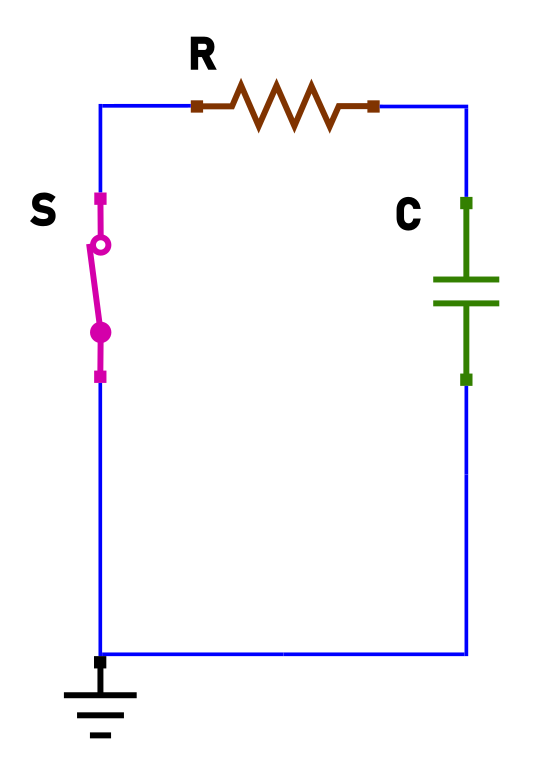
\includegraphics[width=\linewidth]{data/scarica-closed.png}
  \end{subfigure}
  \begin{subfigure}[b]{0.347\linewidth}
    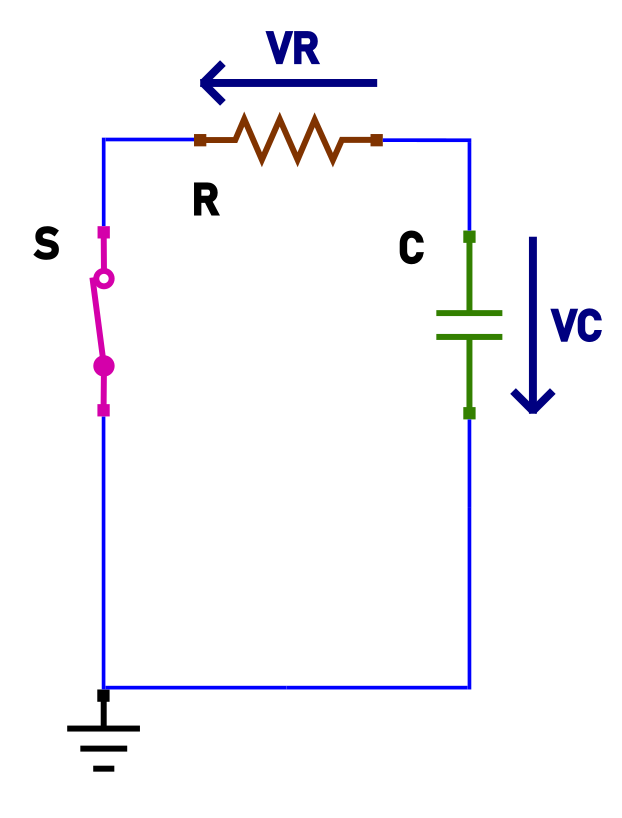
\includegraphics[width=\linewidth]{data/scarica-tensioni.png}
  \end{subfigure}
\end{figure}

\subsubsection*{grafici scarica}

\begin{figure}[h!]
  \centering
  \begin{subfigure}[b]{0.3\linewidth}
    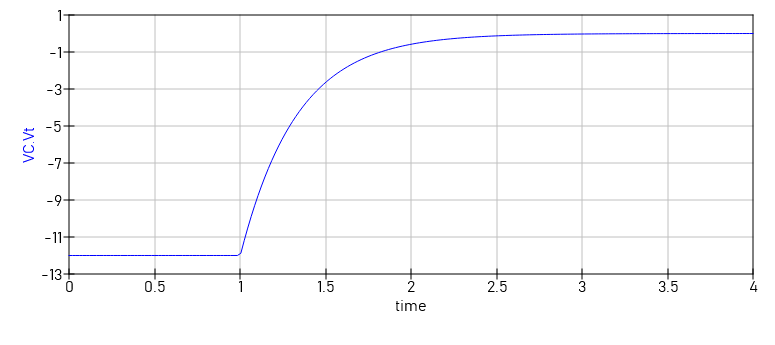
\includegraphics[width=\linewidth]{data/scarica-VC.png}
  \end{subfigure}
  \begin{subfigure}[b]{0.3\linewidth}
    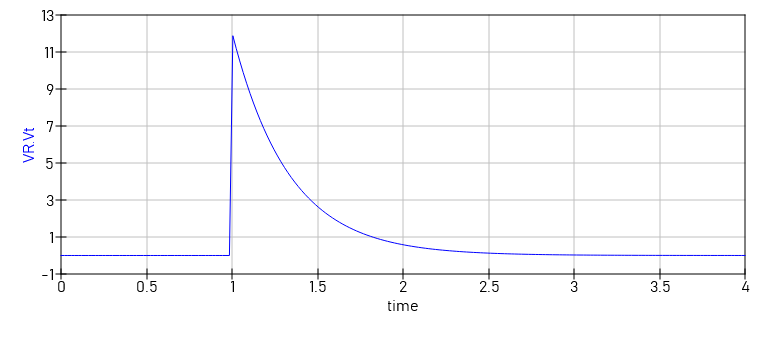
\includegraphics[width=\linewidth]{data/scarica-VR.png}
  \end{subfigure}
  \begin{subfigure}[b]{0.3\linewidth}
    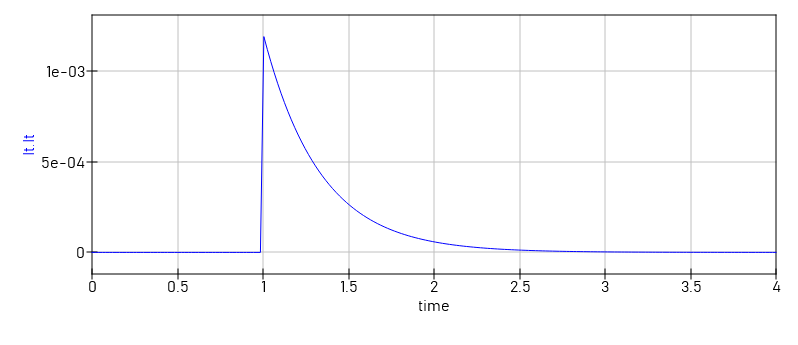
\includegraphics[width=\linewidth]{data/scarica-IT.png}
  \end{subfigure}
\end{figure}

\newpage

\section*{simulazione con qucs}

\subsubsection*{carica}

\begin{figure}[!h]
  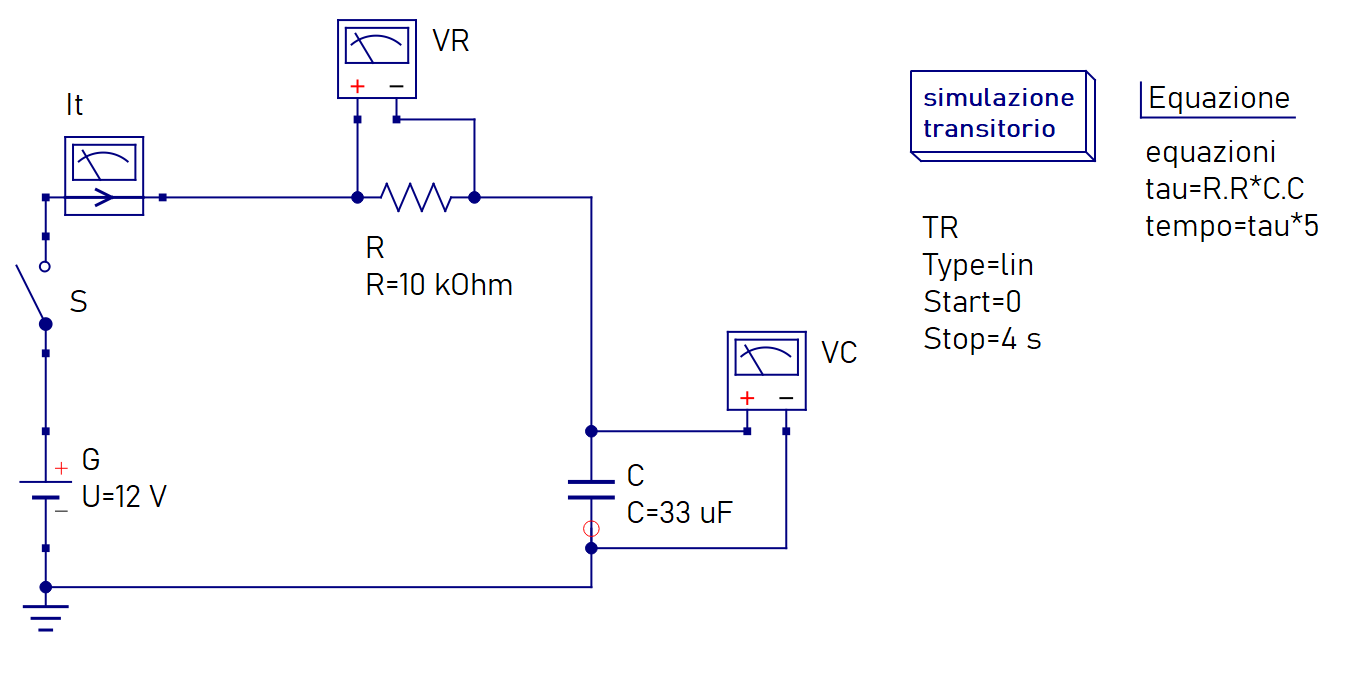
\includegraphics[width=\linewidth]{data/carica-simulazione-qucs.png}
\end{figure}

\subsubsection*{scarica}

\begin{figure}[!h]
  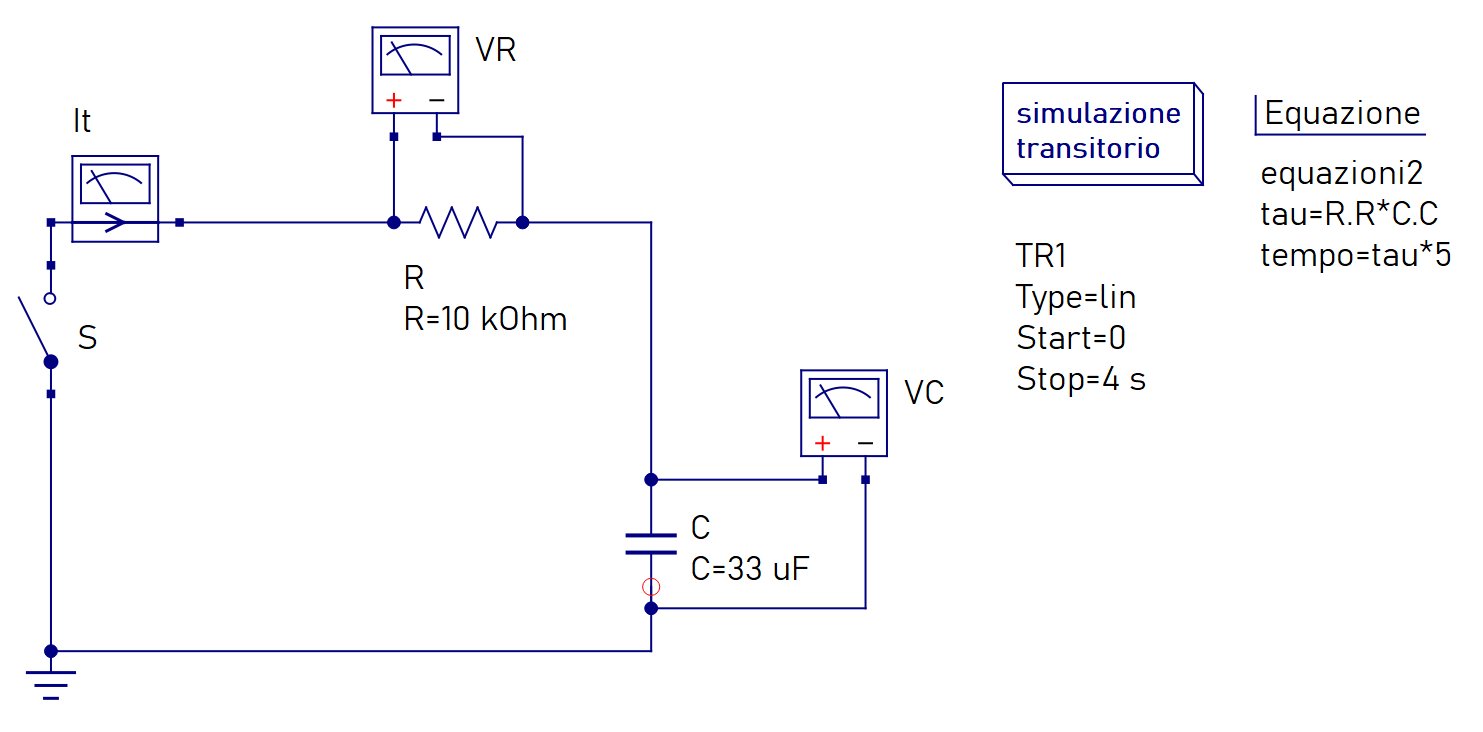
\includegraphics[width=\linewidth]{data/scarica-simulazione-qucs.png}
\end{figure}

\newpage

\section*{conclusioni e osservazioni}
\blindtext[1]


\end{document}